\documentclass[10pt,a4paper]{article} % tamaño de letra y tipo de papel
\usepackage[utf8]{inputenc}
\usepackage[spanish]{babel} % paquete para que reconozca ñ y tildes
\usepackage{amsmath}
\usepackage{amsfonts}
\usepackage{amssymb}
\usepackage{upgreek} 
\usepackage{graphicx} % paquete para incluir imagenes
\usepackage[margin=1in,bottom=1in]{geometry}
\usepackage{hyperref} % paquete para tener marcadores en el pdf
\author{Ulloa Daniel}
\begin{document}

\begin{titlepage}
	\hbox{
		\hspace*{0.15\textwidth} % Espacio desde el margen izquierdo
		\rule{1pt}{\textheight} % Linea decorativa
		\hspace*{0.05\textwidth} % Espacio entre la linea y el texto
		\parbox[b]{0.75\textwidth}{ % Caja que restringe el espacio que puede ocupar el texto
			{\noindent\Huge\bfseries Informe de Laboratorio } % Titulo
			\\ 
			[2\baselineskip] 
			{\large \textbf{Tema:} Oscilador con Resistencia Negativa} % Tema
			\\[4\baselineskip]
            {\large \textbf{Cátedra:} Teoría de Circuitos \textsc{II}} % Catedra
            \\[1\baselineskip]
            {\large \textbf{Año:} 2019} % Año
			\\[1\baselineskip]
            {\large \textit{\textbf{Docentes:} % Docentes
                \textnormal{Ing. Costa}, Nicolás. 
                \textnormal{Aux. Consiglio}, Dante}
            }
			\\[1\baselineskip]
            {\large \textit{\textbf{Alumnos:} % Alumnos
                \textnormal{Rodriguez}, Ana Victoria. 
                \textnormal{Ulloa}, Daniel Alejandro}
            }
            \\[6\baselineskip]
            {\large \textbf{Fecha de Entrega:} 11/09/2019}
			\par %Para que el logo aparezca al pie
			\vspace{0.35\textheight} % Ubicacion de la caja desde el margen superior
            \center{
\includegraphics[width=250px]{logo2.png}}
            \\[1\baselineskip]
	}}
\end{titlepage}
\tableofcontents
\newpage
\section{Introducción}

\section{Objetivos}
\begin{itemize}
    \item Modelar e interpretar el Circuito
    \item Obtener la respuesta temporal de la tensión de salida y graficarla en Mathematica
    \item Realizar un barrido paramétrico sobre la resistencia $R_B$ y observar las diferentes respuestas.
\end{itemize}
\section{Modelado Matemático}
El circuito a modelar se muestra a continuación %sopenca
\begin{center}
%    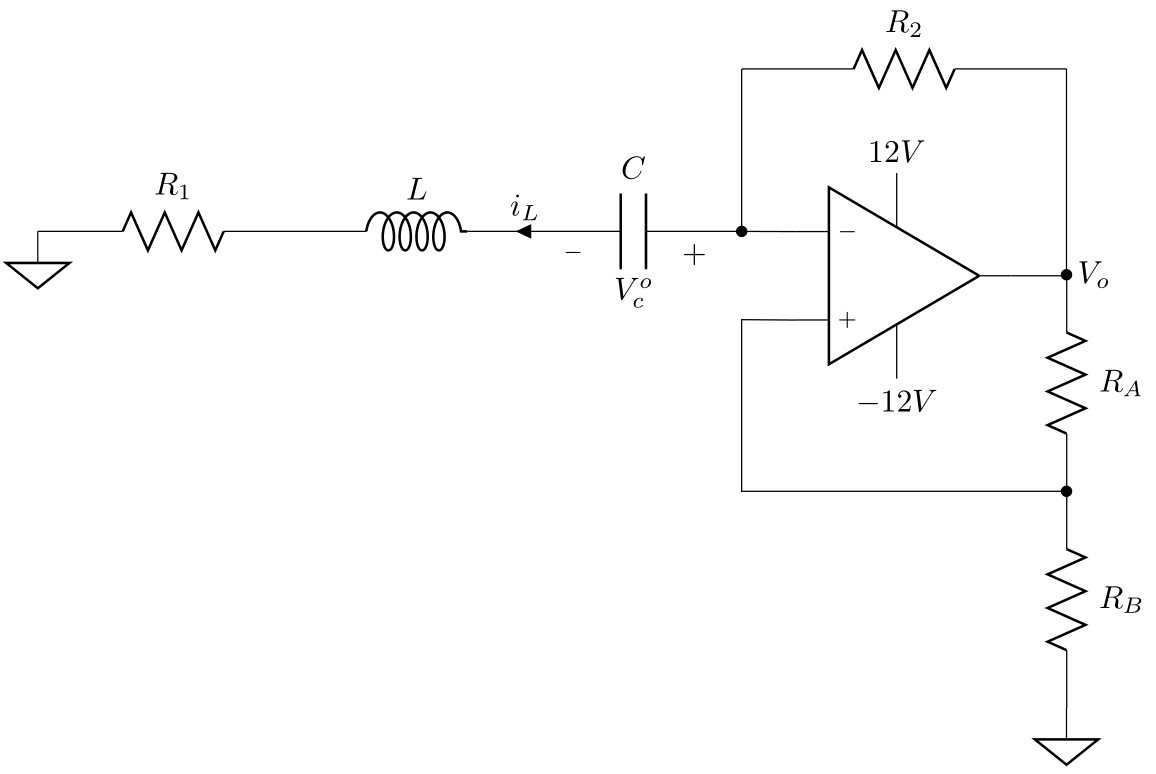
\includegraphics[width=300px]{circuito}
\end{center} 
Se consideró el amplificador operacional ideal y se analizó el nodo $V_{n}$.
Se tiene dos corrientes, la correspondiente al RLC y la que pasa por la resistencia $R_{2}$. \\
\begin{equation}
i(t)=i_{R2}(t)
\end{equation}
Sabiendo que la corriente que pasa por el RLC es la del capacitor dado a que es el elemento con condiciones iniciales, esta es igual a 
\begin{equation}
i(t)=C*V_{c}'(t)
\end{equation}
y la corriente que pasa por la resistencia R2 
\begin{equation}
i_{R2}(t)=\frac{V_{n}(t)-V_{o}(t)}{R_{2}}
\end{equation}
Donde las tensiones $V_{n}(t)$ y $V_{p}(t)$ son iguales al considerar que el amplificador operacional es ideal, y su vez , que  $V_{p}$ es la tensión de un divisor de tensión formado por las resistencias $R_{a}$ y $R_{b}$ y la tensión de salida  $V_{o}(t)$. 

\begin{equation}
V_{p}(t)=\frac{R_{b}* V_{o}(t)}{R_{a}+R_{b}}
\end{equation}
De esta manera se obtiene la primera ecuación de nuestro sistema, a la cual se le aplicó la transformada de Laplace, obteniendo 
\begin{equation}
eq1=C* (s V_{c}(s)-V_{c}(t))+\frac{R_{a}* V_{o}(s)}{R_{2} R_{a} +R_{2} R_{b}}
\end{equation}
Para la segunda ecuación se recorrio la malla que contiene a los componentes $R_{1},R_{2}, C$ y $L$, cuya suma de las tensiones es igual a la tensión en la salida. 
\begin{equation}
\ V_{o}(t)=\ V_{c}(t)+ V_{l}(t)+ V_{r}(t)
\end{equation}
\begin{equation}
V_{o}(t)=C*L*V_{c}''(t)+ C*(R_{1}+R_{2})*V_{o}'(t)+V_{c}(t)
\end{equation}
Nuevamente se aplico la transformada de Laplace, obtiendo la segunda ecuación
\begin{equation}
eq2 = V_{c}(s) - V_{o}(s) + C(R_{1} + R_{2})(s*V_{c}(t) - v_{0}(t)) + 
LC(s^{2}*V_{c}(t) - s*v_{0}(t))
\end{equation}
Con estas dos ecuaciones es posible obtener las tensiones de salida y entrada del sistema y su función de transferencia 
\begin{equation}
H(s)=\frac{C R_{2} (R_{a}+R_{b})}{s*R_{a}C (s*\text{L} +R_{1}+2 R_{2})+s*\text{C}R_{2} R_{b} +R_{a}}
\end{equation}
Reordenando la función de transferencia
\begin{equation}
H(s)=\frac{\frac{CR_{2}*(R_{a}+R_{b})}{R_{a}}}{1+(CR_{1}+2CR_{2}+\frac{CR_{2}R_{b}}{R_{a}})s+(LC)s^{2}}
\end{equation}
\\
Teniendo en cuenta el modelo teórico 
\begin{equation}
H(s)=\dfrac{Y(s)}{U(s)}=\dfrac{K}{s^{2}\tau^{2}+2\xi \tau s+1}
\end{equation}
Adaptando el modelo teórico con el obtenido
\begin{equation}
K=\frac{CR_{2}*(R_{a}+R_{b})}{R_{a}}
\end{equation}
\begin{equation}
\tau=\sqrt{LC}
\end{equation}

\begin{equation}
\xi=\dfrac{1+(CR_{1}+2CR_{2}+\frac{CR_{2}R_{b}}{R_{a}})}{2\sqrt{LC}}
\end{equation}
 Si las resistencias son iguales, el nuevo valor de $\xi$ es 
\begin{equation}
\xi=\dfrac{1+4RC}{2\sqrt{LC}}
\end{equation}
\section{Respuesta Temporal}
Para la respuesta temporal del oscilador aplicamos la %antitransformada o inversa obteniendo 
\begin{equation}
H(t)=d*\dfrac{e^{(-a-\dfrac{\sqrt{b}}{c})t}-e^{(-a+\dfrac{\sqrt{b}}{c})t}}{\sqrt{b}}
\end{equation}

Donde 
\begin{equation}
a=\frac{R_{1}}{2 \text{L}}+\frac{R_{2} R_{b}}{2 \text{L} R_{a}}+\frac{R_{2}}{\text{L}}
\end{equation}
\begin{equation}
b=(\text{C} R_{1} R_{a} +2 \text{C} R_{2} R_{a} +\text{C} R_{2} R_{b})^2-4 \text{C} \text{L} R_{a}^2
\end{equation}
\begin{equation}
c=2 \text{L} \text{C} R_{a}
\end{equation}
\begin{equation}
d= (R_{a}+R_{b})R_{2}C
\end{equation}



\section{Barrido Paramétrico}
\section{Conclusión}
\end{document} 


